\chapter{Emacs Basics}
\section{What is Emacs?}

Emacs is an text editor.


Learning to use an editor is basically a matter of learning finger habit.
Good finger habits can make you an incredibly fast typist.
Intellectually, it's possible to absorb a lot from one reading, but you can form only a few new habit each day.
Don't feel obliged  to learn them all at once; pick something, practice it, and move on to the next topic.
Time spent developing good habits is time well spent.


\section{Why You Should Use Emacs}
There are following reasons to use Emacs:
\begin{itemize}
\item \keyword{Efficiency}: There are many commands that can move cursor without a mouse. There are many commands to help you saving typing.
\item \keyword{Powerful}: It provides many major and minor modes for special situation. I often use the latex mode.
\item \keyword{Extensibility}: If there is some function not meeting your need, you can programm to implement it using Emacs Lisp language.
\end{itemize}



\section{Files and Buffers}
In Emacs, you don't really edit \keyword{files} (stored on disk).
Instead, Emacs copies the content of a file into a temporary \keyword{buffer} and you edit that.
The file on disk doesn't change until you save the buffer.

\section{Modes}
Emacs becomes sensitive to the task at hand.
\keyword{Modes} allows Emacs to the kind of editor you want for different tasks.
A buffer can be in only one \keyword{major mode} at a time.
\keyword{Minor modes} defines a particular aspect of Emacs's behavior and can be turned on and off within a major mode.

If you are good at Lisp programming, you can add your own modes.
Emacs is almost infinitely extensible.


\section{Display}
\label{sec:display}

The display is shown in Figure \ref{fig:display}.

\begin{figure}[!htbp]
  \centering
  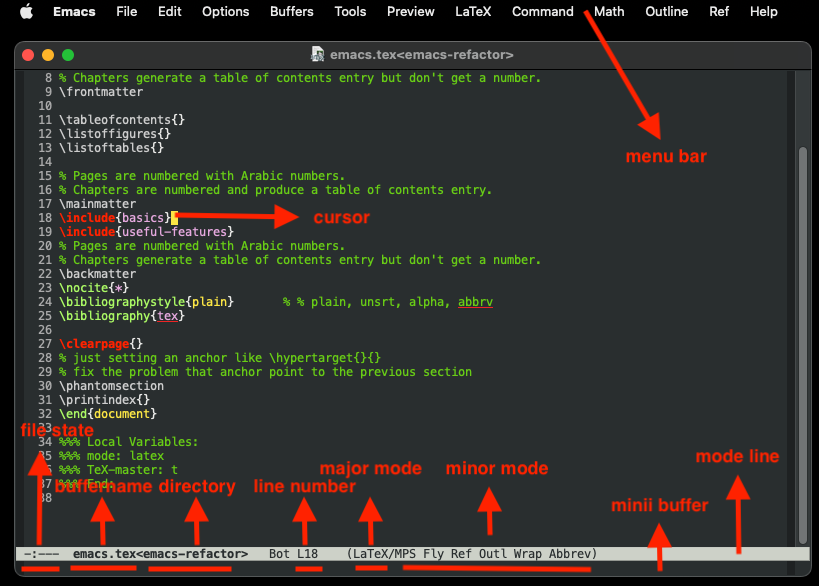
\includegraphics[width=0.9\textwidth]{display}
  \caption{Display}
  \label{fig:display}
\end{figure}


Here I have configured Emacs to hide the tool bar.
The operation is: Options $\longrightarrow$ Show/Hide $\longrightarrow$ Toolbar.
After that, you will see the following file in \argument{~/.emacs}:

\begin{lstlisting}
(custom-set-variables
 '(tool-bar-mode nil))
\end{lstlisting}

The \keyword{mode line} is the place to some useful information.
The \keyword{file state} shows the state of the current buffer.
For example, it is read only or not, altered or not.

\section{Commands}
You issue commands to instruct Emacs to do what you want to.
Each \keyword{command} has a formal name, which is the name of a Lisp routine (Emacs is written with Emacs Lisp language).
Some command names are quite long.
As a result, we need some way to abbreviate commands.
Emacs ties a command name to a short sequence of keystrokes.
This tying of commands to keystrokes is known as \keyword{binding}.


The author of Emacs try to bind the most frequently used commands to the key sequences that are the easiest to reach (\keyword{C: Ctrl, M: Meta}):
\begin{itemize}
\item The most commonly used commands are bound to \keyword{C-n}(where \keyword{n} is any character).
\item Slightly less commonly used commands are bound to \keyword{M-n}.
\item Other commonly used commands are bound to \keyword{C-x keystrokes}.
\item Some specialized commands are bound to \keyword{C-c keystrokes}. These commands often relate to one of the more specialized modes, such as Java or HTML mode.
\item To use commands that is binded, use \keyword{M-x command-name Enter}. (This works for any command really)
\end{itemize}


\section{Kill Ring}
\label{sec:kill-ring}

Emacs use \keyword{kill} commands to delete text, for example \keyword{kill-region, kill-word}.
However, killing is not fatal, but in fact, quite the opposite.
Text that has been killed is not gone forever but is hidden in an area called the \keyword{kill ring}.
The kill ring is an internal storage area where Emacs puts things you’ve copied or deleted.



What exactly goes into the kill ring?
Only the text delete by \keyword{Del} and \keyword{C-d} (without numeric argument) does not go into kill ring. All the else will go into kill ring.


\section{Pointer and Cursor}
\label{sec:pointer-mark}

A \keyword{cursor} is on the top the char.
A \keyword{pointer} is the position between the cursor and one char before the cursor.


\section{Backup Files}
\label{sec:backup-files}

A backup file is a copy of the old contents of a file you are editing.
Emacs makes a backup file the first time you save a buffer into its visited file.
Thus, normally, the backup file contains the contents of the file as it was before the current editing session.
The contents of the backup file normally remain unchanged once it exists.
Thus the backup file keeps a copy of the original file.
During the editing, you may save the buffer several times and the content of the original file will change accordingly.

The name of the backup file is the same as the name of the file you’re editing, with a tilde (\textasciitilde{}) added.
For example, if you are editing the file \argument{text}, the backup file is \argument{text\textasciitilde{}}


\section{Auto Save Files}
\label{sec:auto-save-files}

Emacs will auto save you files from time to time into \argument{auto-save files}.
The name of an auto-save file is the same as the name of the file you are editing, with a sharp (\#) added to the beginning and the end.
For example, if you are editing the file \argument{text}, its auto-save file is \argument{\#text\#}.

The save files are used save the content of current buffer if you do not save the buffer and the Emacs or system crashed.









%%% Local Variables:
%%% mode: latex
%%% TeX-master: "emacs"
%%% End:
